% Diapo d'intro

\begin{frame}[c]
  \frametitle{Context and Aims}

%\todo{À revoir}

\tval{MeForBio} team:\\
\quad \quad Algebraic modelling to study complex dynamical biological systems

%\bigskip
\begin{center}
  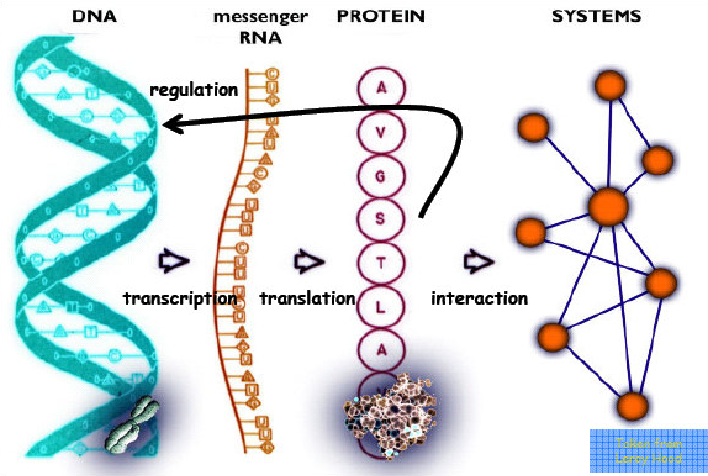
\includegraphics[height=3.5cm]{figs/dnascheme_white.png}
\end{center}

\pause
\begin{enumerate}[1)]
  \item Asynchronous Discrete Networks (ADN)
  \begin{itemize}
    \item[] Convenient to model biological systems
  \end{itemize}

  \smallskip
  \item Process Hitting (PH)
  \begin{itemize}
    \item[] Cannot accurately describe ADNs
  \end{itemize}

  \smallskip
  \item Enhancing PH with priorities
  \begin{itemize}
    \item[] To efficiently compute reachability in ADNs
  \end{itemize}
\end{enumerate}

\end{frame}
